\section{Аналитическая часть}
 
РПЗ НЕ ИНТЕРЕСНО ЧИТАТЬ ПОТОМУ ЧТО НЕТ КОНФЛИКТА.
 
В данном разделе производится анализ предметной области, приводятся методы трансляции, рассматриваются существующие оптимизации трансляции и рассматриваются существующие проблемы.
 
\subsection{Постановка задачи?}
 
Никакой из существующих трансляторов не достигает стопроцентной скорости выполнения программ, хотя теоретически такая скорость достижима.
 
а че еще сказать.......

write

\subsection{Методы трансляции}

write

Надо написать почему он тупит... И все методы типа тупят почему.

\subsubsection{Интерпретация}

Под интерпретацией понимается реализация каждой команды процессора в виде кода на языке высокого уровня. Такой подход обеспечивает высокую точность исполнения, так как обычно описывает все, даже самые малые, изменения в состоянии процессора. Из рассматриваемых методов имеет самую маленькую скорость выполнения, так как исполняющему код процессору приходится постоянно разбирать транслируемый код и выполнять его при помощи вызовов функций.

\subsubsection{Рекомпиляция}

Под рекомпиляцией понимается преобразование машинного кода одной архитектуры в другую. Таким образом после рекомпиляции процессор выполняет родной для себя код без необходимости вызова функций. Не все машинные инструкции имеют точные аналоги на другой архитектуре, так что необходимо хранить дополнительные данные, например ARM не рассчитывает все флаги архитектуры x86 и их необходимо сохранять отдельно. По скорости рекомпиляция быстрее интрепретации.

\subsubsection{Эмуляция высокого уровня}

Под эмуляцией выского уровня понимается подмена каких-либо высокоуровневых функций на их эквиваленты для архитектуры хоста. Например, при эмуляции приложения использующего библиотеку libc можно заменить все вызовы функций этой библиотеки на вызовы функций библиотеки libc хоста, видимый результат функций одинаков, при этом не нужно транслировать или рекомпилировать эти функции. Данный метод не подходит для эмуляции всей системы, однако может сильно повысить производительность если таких вызовов много.

\subsubsection{Сравнение методов трансляции}

Эмуляция высокого уровня сама по себе не может обеспечить эмуляцию всей системы, однако в связке с рекомпиляцией или интерпретацией повышает производительность последних. Интерпретация используется в случаях когда нужно точно испольнять команды процессора, рекомпиляция также может достигнуть такую точность, но для этого нужно проделать намного больше работы.

\subsection{Динамические трансляторы}

Как уже было упомянуто выше для запуска приложений собраных под иную платформу нужно использовать трансляцию. В данном разделе рассматриваются поддерживающие ARM динамические трансляторы QEMU, box64 и FEX. Достоинство динамических трансляторов --- скорость запуска программы, так как трансляции происходит во время выполнения, нет необходимости ждать окончания, например, рекомпиляции.

\subsubsection{QEMU}

QEMU поддерживает эмуляцию как пользовательского режима, так и эмуляцию всей системы. QEMU транслирует машинные инструкции при помощи промежуточного представления, в качестве промежуточного представления используются «TCG ops», по организации похожие на инструкции архитектур RISC, эти операции сначала оптимизируются, а затем выполняются на хосте, таким образом проще портировать TCG на различные платформы. \cite{qemu_readme}

В QEMU реализованы инструкции x86, x86-64, x87, MMX и MMXEXT. 

%Операции поддерживаются над 32 и 64 битными целыми числами, указатели определены как псевдоним над соответствующим целым числом. 
Пример операции TCG представлен на листинге \ref{code:tcg}:

\begin{code}
	\captionof{listing}{Пример операции TCG}
	\label{code:tcg}
	\begin{minted}
		[
		frame=single,
		framerule=0.5pt,
		framesep=20pt,
		fontsize=\small,
		tabsize=4,
		linenos,
		numbersep=5pt,
		xleftmargin=10pt,
		]
		{text}
add_i32 t0, t1, t2  (t0 <- t1 + t2)
	\end{minted}
\end{code}

\subsubsection{box64}

box64 --- эмулятор пользовательского режима, в отличие от QEMU box64 не может эмулировать полную систему, однако может запускать linux-приложения собранные под x86\_64. box64 проводит динамическую трансляцию без использования промежуточного представления, таким образом при динамической рекомпиляции поддерживаемые инструкции, при помощи макросов C, транслируются в инструкции ARM. box64 также включает в себя эмулятор, написанный на C который работает как интерпретатор, используемый при запуске на архитектуре отличной от ARM. \cite{box64_letter}

В box64 реализованы инструкции x86, x86-64, x87 и, частично, MMX, MMXEXT, SSE, SSE2, SSE3. 

Каждый блок транслируется в 4 прохода:
\begin{itemize}[leftmargin=1.6\parindent]
	\item[---] Первый проход считает все количество транслируемых x86 инструкций. Для каждой инструкции выделяется память.
	\item[---] На втором проходе обрабатываются все инструкции ветвления, проверяется где находится адрес: в этом же блоке или в каком-либо другом. В случае если адрес находится в другом блоке его необходимо связать с текущим. Также рассчитываются флаги процессора, не нужные флаги предлагается не рассчитывать, так как инструкция может использовать/выставлять не все флаги.
	\item[---] На третьем проходе считается количество необходимых ARM инструкций в блоке.
	\item[---] На четвертом проходе генерируются необходимые инструкции.
\end{itemize}

После генерации блока он записывается в таблицу сгенерированных блоков, в которой также содержится отображение эмулированных адресов в физические. \cite{box64_wide}

\subsubsection{FEX}

FEX, как и box64, является эмулятором пользовательского режима, в отличии от box64 FEX используется промежуточное представление вида СЕП. FEX поддерживает не оптимизированную трансляцию в x86 и оптимизированную трансляцию в ARM. В FEX реализованы инструкции x86, x86-64, x87, MMX, SSE1, SSE2, SSE3, SSSE3 и BMI. 

Трансляция происходит в 4 этапа:

\begin{itemize}[leftmargin=1.6\parindent]
	\item[---] Frontend: Декодирование инструкций, при декодировании также определяются границы блоков трансляции и функций.
	\item[---] OpDispatcher: Перевод инструкций во внутренние (SSA IR, IR.json) инструкции.
	\item[---] IR/Passes: Оптимизация внутренних инструкций.
	\item[---] JIT: Трансляция внутренних инструкций в машинные инструкции платформы хоста.
\end{itemize}

x86 инструкции декодируются в более простые для обработки, например инструкция add имеет большое количество опкодов, хотя по сути там меняются размеры и типы операндов, а не сама операция. Тогда операции add, представленные на листинге \ref{code:decode}, попадают в одну категорию.

\begin{code}
	\captionof{listing}{Пример декодирования инструкций в FEX}
	\label{code:decode}
	\begin{minted}
		[
		frame=single,
		framerule=0.5pt,
		framesep=20pt,
		fontsize=\small,
		tabsize=4,
		linenos,
		numbersep=5pt,
		xleftmargin=10pt,
		]
		{text}
00 C0: add al, al
04 01: add al, 0x1
	\end{minted}
\end{code}

Использование СЕП облегчает оптимизацию кода, например, при устранении бессмысленных присвоений, которые показаны в листинге \ref{code:why_assign}:

\begin{code}
	\captionof{listing}{Пример лишнего присваивания}
	\label{code:why_assign}
	\begin{minted}
		[
		frame=single,
		framerule=0.5pt,
		framesep=20pt,
		fontsize=\small,
		tabsize=4,
		linenos,
		numbersep=5pt,
		xleftmargin=10pt,
		]
		{text}
y := 1
y := 2
x := y
	\end{minted}
\end{code}

Не сложно понять, что первое присвоение переменной не нужно, однако для транслятора это далеко не так очевидно. Пример использования СЕП на листинге \ref{code:SSA}:

\begin{code}
	\captionof{listing}{Использование СЕП для определения бессмысленных присвоений}
	\label{code:SSA}
	\begin{minted}
		[
		frame=single,
		framerule=0.5pt,
		framesep=20pt,
		fontsize=\small,
		tabsize=4,
		linenos,
		numbersep=5pt,
		xleftmargin=10pt,
		]
		{text}
y1 := 1
y2 := 2
x1 := y2
	\end{minted}
\end{code}

СЕП решает следующие задачи:
\begin{itemize}[leftmargin=1.6\parindent]
	\item[---] свёртка констант;
	\item[---] удаление мёртвого кода;
	\item[---] частичное устранение избыточности;
	\item[---] снижение стоимости операций;
	\item[---] распределение регистров.
\end{itemize}

После трансляции в IR количество инструкций больше изначального в 10-30 раз, так как, например, в соответствии с СЕП для каждого присваивания генерируются новые переменные. 32-х битные инструкции расширяются до 64 бит.

write (write what?)

\subsubsection{Сравнение динамических трансляторов}

write

Рассмотрим два аспекта динамических трансляторов, скорость и полноту трансляции.

Для замеров скорости использовался однопоточный бенчмарк nbench.

\begin{figure}[hbtp]
	\centering
	\begin{tikzpicture}  
		\begin{axis}  
			[ 
			height = 9cm,
			width = 12cm,
			ybar,
			enlarge x limits=0.15,
			enlarge y limits=0.03,
			ymax=80,
			ylabel={Производительность},
			symbolic x coords={native, box64, QEMU, FEX},  
			xtick=data,  
			]  
			\addplot coordinates {(native, 79.279) (box64, 34.795) (QEMU, 20.143) (FEX, 15.03)};
			\addplot coordinates {(native, 51.225) (box64, 28.833) (QEMU, 6.893) (FEX, 17.192)};
			\legend{integer, float}  
		\end{axis}  
	\end{tikzpicture}\\
	\caption{Результаты замеров}
	\label{fig:speed}
\end{figure}

Таким образом видно что динамический транслятор box64 достигает 44\% скорости целочисленных вычислений и 56\% вычислений с плавающей точкой. Используя только критерий скорости, можно сделать вывод что он является лучшим решением для динамической трансляции. Однако, по полноте трансляции он сильно проигрывает двум другим трансляторам: box64 не может транслировать все загружаемые библиотеки, то есть для корректной работы он почти обязательно будет использовать родные для архитектуры библиотеки, что целиком обходит проблему именно трансляции. Также, box64 не может рекомпилировать бинарные файлы созданные только на языке ассемблера, он их интерпретирует. Наконец, box64 не поддерживает все SIMD-операции и не умеет правильно докладывать о доступных расширениях процессора через CPUID. Таким образом box64 достаточно далек от полноценного решения для трансляции. (адский главред)

QEMU достигает 25\% скорости целочисленных вычислений и 13\% вычислений с плавающей точкой. Пипец...

FEX достигает 18\% скорости целочисленных вычислений и 33\% вычислений с плавающей точкой. норм)

\begin{table}[!htb]
	\label{table:methods}
	\begin{center}
		\caption{Таблица результатов отдельных бенчмарков.}
		\begin{tabular}{|c|c|c|c|c|}
			\hline
			\bfseries Бенчмарк & \bfseries native & \bfseries box64 & \bfseries QEMU & \bfseries FEX  \\
			\hline
			NUMERIC SORT & 831.84 & 421.07 & 300.83 & 211.29 \\ \hline
			STRING SORT & 413.19 & 209.33 & 57.525 & 25.112 \\ \hline
			BITFIELD & 258910000 & 216760000 & 92293000 & 56201000 \\ \hline
			FP EMULATION & 370.51 & 111.52 & 102.89 & 41.368 \\ \hline
			FOURIER & 56443 & 33655 & 1946.3 & 9898.4 \\ \hline
			ASSIGNMENT & 22.622 & 12.22 & 7.1951 & 9.7578 \\ \hline
			IDEA & 7196.3 & 2016.5 & 1228.8 & 1660.5 \\ \hline
			HUFFMAN & 2396.6 & 859.58 & 625.73 & 566.98 \\ \hline
			LU DECOMPOSITION & 1261.4 & 401.87 & 91.377 & 280.59 \\ \hline
		\end{tabular}
	\end{center}
\end{table}

Из нее можно заметить что ФЕКС когда в память лазит начинается ЛАГАЛОВО)

\subsection{Существующие оптимизации трансляции}

write

\subsubsection{Использование блоков трансляции}

Блоки трансляции используются в каждом из рассматриваемых трансляторов.

В QEMU как блок трансляции выделяется часть кода до момента изменения состояния процессора которое нельзя выяснить на этапе трансляции, например, некоторое ветвление. \cite{qemu_docs}

В box64, так же как и в QEMU, код разбивается на блоки трансляции, блок заканчивается когда после нее нет других инструкций, например jump, call или ret, и когда на последнюю инструкцию не ссылается ветвление из этого блока. Исключением являются многобайтовые NOP инструкции, которые обрабатываются отдельно, а прочтение неизвестной инструкции останавливает выполнение блока. \cite{box64_letter}

В FEX Frontend.cpp разбивает код на блоки трансляции. Блок так же заканчивается при изменении порядка выполнения, однако рассматривается ситуация когда блоки трансляции находятся в одном месте. Некоторые трансляторы заканчивают трансляцию при изменении порядка выполнения, хотя в скомпилированном коде часто встречаются конструкции похожие на листинг \ref{code:compiled}:

\begin{code}
	\captionof{listing}{Пример кода, сгенерированного компилятором}
	\label{code:compiled}
	\begin{minted}
		[
		frame=single,
		framerule=0.5pt,
		framesep=20pt,
		fontsize=\small,
		tabsize=4,
		linenos,
		numbersep=5pt,
		xleftmargin=10pt,
		]
		{text}
test eax, eax
jne .Continue
ret           <--- Можно продолжать трансляцию после 
                   безусловного окончания функции
.Continue:
	\end{minted}
\end{code}

Если можно определить адрес условного перехода, то есть возможность продолжить трансляцию. \cite{fex_front}

Одной из важных оптимизаций является связывание различных блоков трансляции. Если не связывать блоки необходимо выходить из цикла выполнения кода, проходить эпилог процедуры и затем искать следующий, необходимый блок.

Например, после выполнения одного блока трансляции QEMU ищет следующий блок, для этого используется PC (эмулируемый program counter) и другая информация о статусе процессора (например регистр CS). Сначала блок ищется в кэше трансляции, если он там не найден он достается из хэш-таблицы и добавляется в кэш. Для поиска нужно выйти из цикла выполнения блока, пройти через эпилог процедуры, найти следующий блок, запустить его, пройдя через пролог процедуры. В качестве оптимизации предлагается связывать несколько блоков трансляции напрямую.

Для этого в конце блока вызывается tcg\_gen\_lookup\_and\_goto\_ptr(), он в свою очередь вызывает helper\_lookup\_tb\_ptr который ищет нужный блок и генерирует инструкцию goto\_ptr, которая либо продолжит управление в нужном блоке, либо вернется в основной цикл трансляции. Похожая оптимизация используется при ветвлении, если ветвление происходит напрямую, в пределах одной страницы QEMU выполняет поиск блока трансляции на который будет произведено ветвление, а затем сохраняет его адрес в транслированном коде, использование данного метода повышает скорость выполнения на ~15\%. Таким образом при следующем выполнении этого блока нет необходимости в поиске следующего блока. \cite{qemu_docs}

В box64 и FEX применяется похожая идея, таким образом сильно снижается время поиска следующего блока при безусловном ветвлении, например в FEX при выполнении 500 миллионов ветвлений поиск блока выполнялся 100 миллионов раз. \cite{fex_video}

\subsubsection{Поддержка специфичных для архитектуры библиотек}

Одним из важных механизмов, позволяющим добиться хорошей производительности, является использование специфичных для архитектуры библиотек. Такой подход используется в box64 и FEX. Например, в box64 в графически требовательных приложениях производительность близка к 100\%, однако в приложениях не использующие сторонние библиотеки (то есть полностью транслируемые) производительность около 50\%.

При эмуляции Quake 3 в box64 (графического приложения с повторно вызываемыми функциями) производительность была около 85\%.

Необходимые для работы приложения библиотеки либо транслируются, либо используется специфичная для архитектуры библиотека (в таком случае производительность выше). Вызовы функций перехватываются для вызова специфичных для архитектуры функций. 

В ELF содержатся специальные символы называемые перемещениями, они используются при линковке для установки адреса необходимой функции. При вызове родной функции в качестве адреса выставляется адрес заранее подготовленного кода, он состоит из последовательности байт \texttt{CC 53 43} и следующими за ней двух указателей. Первый указатель рассматривается как указатель на оберточную функции, а второй как указатель на обертываемую (родную) функцию. Оберточной функции передается структура с состоянием процессора и указатель на вызываемую функцию, эта структура распаковывается и вызывается переданная функция. По завершению работы оберточная функции завершается через ret или retn.

Поиск необходимой функции осуществляется при помощи файлов находящихся в src/wrapped, их необходимо определять в ручную, так как названия функций не сохраняются после компиляции программы. Сигнатура функции состоит из символов, определяющих тип возвращаемого значения и типов аргументов, разделенных буквой F. Пример сигнатуры показан на рисунке \ref{fig:box64sig}.

\begin{figure}[hbtp]
	\centering
	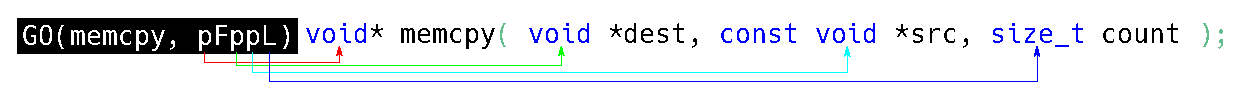
\includegraphics[width=\textwidth]{img/function.eps}
	\caption{Пример сигнатуры функции memcpy}
	\label{fig:box64sig}
\end{figure}

После определения функция заносится в таблицу функций библиотеки, а затем находится при помощи разных методов. \cite{box64_deep}

В FEX так же существует поддержка специфичных для архитектуры библиотек, но, например, используется другая последовательность байт --- \texttt{0F 36}, реализация похожа на реализацию в box64.

\subsubsection{Оптимизации кода}

В FEX и QEMU реализованы некоторые оптимизации, свойственные оптимизирующим компиляторам, критерием выбора оптимизаций является скорость работы (так как трансляция динамическая) и эффективность.

box64 является меньшим проектом, поэтому в нем реализовано меньше оптимизаций кода.

Программы собранные под архитектуру x86 не работают на таких компьютерах, необходим или статический транслятор, такой как Rosetta 2, или виртуальная машина поддерживающая необходимую архитектуру. Rosetta 2 не транслирует программы не предназначенные для macOS, для запуска программ созданных для Windows или Linux нужно использовать виртуальную машину. Еще одно ограничение статической трансляции --- наличие самомодифицирующегося кода и динамических библиотек, таким образом использование только статической трансляции не запустит любую программу. \cite{fast_bin}

\subsubsection{Распространение констант}

При этом проходе заменяется выражение, которое при выполнении всегда возвращает одну и ту же константу, самой этой константой. Это значение прописывается в инструкцию.

\subsubsection{Устранение мертвого кода}

Устраняется <<бессмысленный>>, не вызываемый код.
Например, на листинге \ref{code:dumb} представлена бессмысленная операция:
\begin{code}
	\captionof{listing}{Пример бессмысленной инструкции}
	\label{code:dumb}
	\begin{minted}
		[
		frame=single,
		framerule=0.5pt,
		framesep=20pt,
		fontsize=\small,
		tabsize=4,
		linenos,
		numbersep=5pt,
		xleftmargin=10pt,
		]
		{text}
  and_i32 t0, t0, $0xffffffff
	\end{minted}
\end{code}

При выполнении побитовой операции И, в которой один из аргументов равен максимально возможному для регистра числу, второй аргумент не изменит значение.

В FEX так же устраняются бессмысленные и ненужные операции.

\subsubsection{Устранение загрузок контекста}

В FEX устраняются бесполезные загрузки контекста, например, если идет сохранение контекста, а затем сразу же его загрузка, такая загрузка выполнятся не будет. 

\subsubsection{Устранение хранения}

В QEMU удаляются неиспользуемые перемещения данных, например, в листинге \ref{code:unused} представлен пример не оптимизированного хранения:

\begin{code}
	\captionof{listing}{Пример не оптимизированных TCG инструкций}
	\label{code:unused}
	\begin{minted}
	[
	frame=single,
	framerule=0.5pt,
	framesep=20pt,
	fontsize=\small,
	tabsize=4,
	linenos,
	numbersep=5pt,
	xleftmargin=10pt,
	]
	{text}
add_i32 t0, t1, t2
add_i32 t0, t0, $1
mov_i32 t0, $1
	\end{minted}
\end{code}

После оптимизации выполнится только последняя инструкция.

В FEX устраняются бесполезные хранения, не высчитываются неиспользуемые флаги (например, те что будут перезаписаны следующей инструкцией: при операции умножения или деления используют несколько регистров и один из этих регистров будет перезаписан следующей инструкцией), если после ветвления в любом случае перезаписывается какое-либо значение --- его можно не хранить.

\subsubsection{Сжатие инструкций}

Многие x86 инструкции читают или записывают регистры подряд, можно объединять их в пары (и использовать ld2 или st1 и подобные).

Некоторые MMX операции (то есть с операндами в 64 бита) можно объединить в операции с операндами в 128 бит которые смогут использовать целый SIMD-регистр архитектуры ARM.

\begin{comment}

\subsubsection{Устранение длинного деления}

Можно устранять длинное деление. Сложноватто короче

\subsubsection{Статическое выделение регистров}

На ARM можно использовать регистровый файл, если все правильно определить регистры можно заменять store context на store registers (уточнить (может это вообще не оптимизация)).
\end{comment}

\subsubsection{Устранение временных регистров}

В FEX, если транслируется блок, который включает в себя весь код функции, и известен используемый двоичный интерфейс, есть возможность исключить временные регистры при сохранении контекста. Также при трансляции целой функции можно убрать загрузки и сохранения в контекст посреди функции и выполнять одно сохранение в конце функции и загрузку в начале.

\subsubsection{Анализ живости}

В QEMU каждый регистр проверяется на используемость в определенном блоке трансляции. Если регистр не используется в блоке трансляции связанные с ним операции оптимизируются, так как значения этих регистров (и связанное с ними состояние процессора) за блок не могут измениться. Если состояние виртуального процессора меняется, такой блок не будет выполняться пока состояние процессора не будет соответствовать необходимому для блока (например, другой уровень привилегий).

Например, если на x86 регистры SS, DS и SS содержат в себе 0, транслятор не будет генерировать для них смещение.

\subsubsection{Сравнение оптимизаций трансляции}

В таблице 1 %\ref{ass}
перечислены выделенные методы трансляции. 

\begin{table}[!htb]
	\label{table:methods}
	\begin{center}
		\caption{Таблица методов трансляции.}
			\begin{tabular}{|c|c|c|c|}
				\hline
				\bfseries Методы & \bfseries QEMU & \bfseries box64 & \bfseries FEX  \\
				\hline
				Промежуточное представление & + & - & + \\ \hline
				Блоки трансляции & + & + & + \\ \hline
				Связывание блоков трансляции & + & + & + \\ \hline
				Поддержка самомодифицирующегося кода & + & + & $\pm$ \\ \hline
				Поддержка родных библиотек & - & + & + \\ \hline
				Распространение констант & + & - & + \\ \hline
				Устранение мертвого кода & + & - & + \\ \hline
				Устранение загрузок контекста & - & - & + \\ \hline
				Устранение хранения & + & - & + \\ \hline
				Сжатие инструкций & + & - & + \\ \hline
				Устранение временных регистров & - & - & + \\ \hline
				Анализ живости & + & - & + \\ \hline
		\end{tabular}
	\end{center}
\end{table}

\newpage

\subsection{Поддержка самомодифицирующегося кода}

Самомодифицирующийся код на x86 представляет особую проблему, так как нет механизма оповещения об изменении кода, в отличие, например, от ARM.

При запуске в режиме пользователя QEMU помечает все страницы с транслированным кодом как защищенные от записи, при попытке записи в них поднимается сигнал SEGV, допускается запись, транслированная страница и связанные с ней блоки помечаются как не валидные. При запуске эмуляции системы программный MMU выполняет защиту от записи и инвалидацию страниц. \cite{qemu_docs}

В box64 используется похожий механизм, все транслированные страницы помечаются защищенными на запись, при попытке попытке записи страница в которую произведена запись и все последующие помечаются как "грязные". Однако, они не обязательно являются невалидными, при попытке выполнения кода с такой страницы считается CRC32, полученный результат сравнивается с контрольной суммой посчитанной при создании блока, если суммы совпадают блок объявляется валидным и опять защищается от записи, иначе генерируется новый блок. \cite{box64_letter}

В FEX не реализована полноценная поддержка самомодифицирующегося кода, по мнению разработчиков подход QEMU и box64 является единственным приемлемым по скорости и планируется использовать его. \cite{FEX_letter}

\subsection{Поддержка TSO}

При трансляции между двоичного кода между платформами следует также учитывать различные модели доступа к памяти, их делят на две группы: слабую и сильную. К слабой модели относятся архитектуры ARM, PowerPC, RISC-V и т.д; к сильной относятся x86/64 и специальные режимы работы процессоров архитектуры SPARC и RISC-V и другие. В таблице \ref{table:memmodels} представлены оптимизаций доступа к памяти на стадии выполнения.

\begin{table}[!htb]
	\begin{center}
		\label{table:memmodels}
		\caption{Таблица переупорядочиваний обращений к памяти \cite{memry}}
		\resizebox{\columnwidth}{!}{%
			\begin{tabular}{|c|c|c|c|c|}
				\hline
				\bfseries  & \bfseries ARMv7-A/R & \bfseries RISC-V (WMO) & \bfseries RISC-V (TSO) & \bfseries x86 \\
				\hline
				Чтение может быть переставлено после чтения  		& Да & Да & - & - \\ \hline
				Чтение может быть переставлено после записи  	& Да & Да & - & - \\ \hline
				Запись может быть переставлена после записи  	& Да & Да & - & - \\ \hline
				Запись может быть переставлена после чтения 	& Да & Да & Да & Да \\ \hline
				Атомарные операции могут быть переставлены с чтением	& Да & Да & - & - \\ \hline
				Атомарные операции могут быть переставлены с записью 	& Да & Да & - & - \\ \hline
			\end{tabular}
		}
	\end{center}
\end{table}

\newpage

Как видно из таблицы, слабые модели памяти включают в себя большее количество перестановок операций. 
\begin{comment}
Рассмотрим приложение созданное для определения количества одного из видов перестановок --- запись переставленная после чтения. 

Написать про суть проги, из цитаты взять

На рисунке \ref{fig:ree} представлено количество перестановок за 1000000 вызовов функций. \cite{reorder}

\begin{figure}[hbtp]
\centering
\begin{tikzpicture}  
\begin{axis}  
[ 
height = 9cm,
width = 12cm,
ybar,
enlarge x limits=0.15,
enlarge y limits=0.004,
ymax=1500,
ylabel={Количество перестановок},
symbolic x coords={Cortex-A53, Cortex-A72, Exynos M2, Apple M1},  
xtick=data,  
]  
\addplot coordinates {(Cortex-A53, 2.4) (Cortex-A72, 1234) (Exynos M2, 427) (Apple M1, 1450)};
%\legend{str}  
\end{axis}  
\end{tikzpicture}\\
\caption{Пример рисунка}
\label{fig:ree}
\end{figure}

На рисунке заметно что ядро Cortex-A53 практически не выполняло перестановки, это связано с тем что оно было выпущено в 2012 году как энергоэффективное ядро, таким образом оно не включает в себя полноценное внеочередное исполнение, только имея возможность одновременного исполнения некоторых команд.
\end{comment}
Таким образом дословная трансляция машинных операций многопоточного приложения с большой вероятностью приведёт к некорректным результатам. 

Простейшее решением этой проблемы --- использование инструкций с барьером. Такие инструкции устанавливают строгую последовательность между обращениями к памяти до и после барьера. Это означает, что все обращения к памяти перед барьером выполнятся до первого обращения к памяти после барьера, если все инструкции доступа к памяти будут выполнятся как инструкции с барьером, невозможна будет ситуация с перестановкой данных.

Использование инструкций с барьером оказывает сильное влияние на производительность ядер с развитой системой внеочередного исполнения, рассмотрим пример программы на ассемблере ARM:

\begin{code}
	\captionof{listing}{Простая программа}
	\label{code:simple}
	\begin{minted}
		[
		frame=single,
		framerule=0.5pt,
		framesep=20pt,
		fontsize=\small,
		tabsize=4,
		linenos,
		numbersep=5pt,
		xleftmargin=10pt,
		]
		{text}
.globl _start
_start:
    mov     x0, 58368
    movk    x0, 0x540b, lsl 16
    movk    x0, 0x2, lsl 32
loop:
    mov     x21, #0xffffffffffffffec
    add     x21, sp, x21
    str     w20, [x21]

    sub     x0, x0, #1
    cmp     x0, 0
    bne     loop

    mov     x0, #0
    mov     w8, #93
    svc     #0
	\end{minted}
\end{code}

Эта программа 10000000000 раз производит сохранение регистра w20 в область памяти стека. Таким образом на время выполнения программы в сильнее всего влияет операция \texttt{str w20, [x21]}. Проведём замеры выполнения программы с операцией \texttt{str w20, [x21]} и с операцией \texttt{stlr w20, [x21]} --- доступом к памяти с барьером. Результаты замеров времени выполнения программы представлены на рисунке \ref{fig:speed}.

\begin{figure}[hbtp]
	\centering
	\begin{tikzpicture}  
		\begin{axis}  
			[ 
			height = 9cm,
			width = 12cm,
			ybar,
			enlarge x limits=0.15,
			enlarge y limits=0.03,
			ymax=110,
			ylabel={Выполнение программы, с},
			symbolic x coords={Cortex-A53, Cortex-A72, Exynos M2, Apple M1},  
			xtick=data,  
			]  
			\addplot coordinates {(Cortex-A53, 42.39) (Cortex-A72, 11.15) (Exynos M2, 10.35) (Apple M1, 3.13)};
			\addplot coordinates {(Cortex-A53, 49.46) (Cortex-A72, 105.58) (Exynos M2, 51.58) (Apple M1, 3.13)};
			\legend{str, stlr}  
		\end{axis}  
	\end{tikzpicture}\\
	\caption{Пример рисунка}
	\label{fig:speed}
\end{figure}

На рисунке видно что ядро Cortex-A53 не сильно пострадало из-за замены операции чтения на операцию чтения с барьером, это связано с тем что его выпустили в 2012 году как энергоэффективное ядро, таким образом оно не включает в себя полноценное внеочередное исполнение, только имея возможность одновременного исполнения некоторых команд. Так же видно что барьерный доступ к памяти для процессоров Cortex-A72 и Exynos M2 является затратной операцией, время выполнения программы вырастает в 10 и в 5 раз соответственной. Для процессора Apple M1 время выполнения этой программы не изменилось, однако барьерный доступ к памяти в нем также связан с потерями в производительности. Отношение времени выполнения барьерных инструкций к обычным как правило падает в новых ядрах.

Несмотря на большую потерю в производительности FEX обрабатывает любой доступ к памяти, кроме доступа к памяти через регистр стека, как доступ к памяти с барьером, это простое, но не производительное решение.

Инженеры компании Apple столкнулись с такой же проблемой и решили ее при помощи специального режима работы своего процессора. Процессоры M1 имеют специальный режим работы, не описанный в спецификации ARM, в этом режиме работы процессор придерживается строгой модели памяти, однако этот режим невозможно включить со стороны пользователя без расширений ядра, которые Apple не рекомендует использовать.

\subsection{Оценка скорости работы трансляторов}

write

\subsection{Вывод}

В данном разделе были рассмотрены некоторые методы трансляции применяемые в среде открытого программного обеспечения. По результатам анализа FEX является наиболее полным решением для трансляции кода, однако его производительность является самой низкой из рассмотренных трансляторов.

\begin{comment}
\subsubsection{Сворачивание и оптимизация тривиальных выражений}

\subsubsection{Состояние процессора и блоки трансляции}


\subsubsection{Поддержка самомодифицирующегося кода}

\subsection{box64}

box64 это норм написать что такое

Одной из оптимизаций в box64, по сравнению с box86 (32-х битной версией эмулятора), является определение простых функций, такие функции не нуждаются в оберточной функции и вызываются напрямую, тем самым экономя время

\subsection{FEX}

\subsection{OpDispatcher}

Внутри FEX используется промежуточное представление, эти команды напоминают ARM64. Так как набор различных инструкций x86 слишком велик (более 1000) предлагается сначала переводить их в IR, а затем оптимизировать. На этом этапе обрабатываются особенности x86 (например MOVSB и подобные инструкции разворачиваются в циклы). OpDispatcher не выделяет регистры. 

\subsection{Трансляция IR в инструкции хоста, JIT}

При трансляции также используется кэш, для каждого потока кэш свой что приводит к избыточности, зато нет проблемы синхронизации. (это шок вообще мне надо писать про организацию кэшей в FEX?)
И еще есть LookupCache, это адреса? (вроде)
(External/FEXCore/Source/Interface/Core/LookupCache.cpp, используется в Arm64Dispatcher.cpp)

Третий уровень используется для реконструкции второго уровня в случае переполнения. Первый уровень не переполняется (разработчик так говорит).

\end{comment}

\begin{comment}
\subsection{ДАЛЬШЕ МОЖНО НЕ ЧИТАТЬ}

Список:

\begin{itemize}[leftmargin=1.6\parindent]
	\item[---] первое;
	\item[---] второе;
	\item[---] пятое;
	\item[---] десятое.
\end{itemize}

Формула:

\begin{equation}
c^2 = a^2 + b^2
\end{equation}

Ссылаемся на рисунок \ref{fig:a1}. Информация из источника \cite{golang}.

\begin{figure}[hbtp]
	\centering
	
\includegraphics[width=\textwidth]{img/golang.png}
	\caption{Пример рисунка}
	\label{fig:a1}
\end{figure}

\begin{code}
	\captionof{listing}{Пример кода}
	\label{code:1}
	\inputminted
	[
	frame=single,
	framerule=0.5pt,
	framesep=20pt,
	fontsize=\small,
	tabsize=4,
	linenos,
	numbersep=5pt,
	xleftmargin=10pt,
	]
	{text}
	{code/main.go}
\end{code}
\end{comment}

\pagebreak